\documentclass{thesisclass}

%% Bibstyle %%
\usepackage[numbers]{natbib}
\usepackage{float}
\usepackage{multirow}
\usepackage{listings}
\usepackage{placeins}
\usepackage{graphicx}
% My OWN PACKAGES %
\usepackage[T1]{fontenc}
\usepackage[ngerman]{babel}
%Predefined paths%
\graphicspath{ {images/} }
%My own predefined paths%

%% Glossar %%
\usepackage[toc,nonumberlist]{glossaries}
\makeglossaries

\lstset{language=Java,
   basicstyle=\small,
   keywordstyle=\color{blue!80!black!100},
   identifierstyle=,
   commentstyle=\color{green!50!black!100},
   stringstyle=\ttfamily,
   breaklines=true,
   %numbers=left,
   numberstyle=\small,
   %frame=single,
   backgroundcolor=\color{blue!3}
} 
\renewcommand*{\lstlistingname}{Quelltextausschnitt}


% Based on thesisclass.cls of Timo Rohrberg, 2009
% ----------------------------------------------------------------
% Thesis - Main document
% ----------------------------------------------------------------

%% ---------------------------------
%% | Information about the thesis  |
%% ---------------------------------

\newcommand{\myname}{Weinmann Philipp}
\newcommand{\mytitle}{Maschinelles Lernen im Kontext der Programmierung natürlicher Sprachen}
\newcommand{\myinstitute}{Institut f\"ur Programmstrukturen\\
											und Datenorganisation (IPD)}
											
\newcommand{\advisor}{Dipl. Inform. Alexander Wachtel}

%\newcommand{\timestart}{Startdatum}
%\newcommand{\timeend}{Enddatum}
\newcommand{\submissiontime}{[FILL OUT DATE HERE]}


%% -------------------------------
%% |  Information for PDF file   |
%% -------------------------------
\hypersetup{
 pdfauthor={\myname},
 pdftitle={\mytitle},
 pdfsubject={Not set},
 pdfkeywords={Not set}
}

%%%%%%%%%%%%%%%%%%%%%%%%%%%%%%%%%
%% Here, main documents begins %%
%%%%%%%%%%%%%%%%%%%%%%%%%%%%%%%%%
\begin{document}

% Describe separation hints here: %
%% --------------------------------
%% | Settings for word separation |
%% --------------------------------
% Help for separation:
% In german package the following hints are additionally available:
% "- = Additional separation
% "| = Suppress ligation and possible separation (e.g. Schaf"|fell)
% "~ = Hyphenation without separation (e.g. bergauf und "~ab)
% "= = Hyphenation with separation before and after
% "" = Separation without a hyphenation (e.g. und/""oder)

\hyphenation{
Sprach-ein-ga-ben
}

\selectlanguage{ngerman}
\floatname{algorithm}{Algorithmus}

\frontmatter
\pagenumbering{roman}
%% titlepage.tex
%%

% coordinates for the bg shape on the titlepage
\newcommand{\diameter}{20}
\newcommand{\xone}{-15}
\newcommand{\xtwo}{160}
\newcommand{\yone}{15}
\newcommand{\ytwo}{-253}

\begin{titlepage}
% bg shape
\begin{tikzpicture}[overlay]
\draw[color=gray]  
 		 (\xone mm, \yone mm)
  -- (\xtwo mm, \yone mm)
 arc (90:0:\diameter pt) 
  -- (\xtwo mm + \diameter pt , \ytwo mm) 
	-- (\xone mm + \diameter pt , \ytwo mm)
 arc (270:180:\diameter pt)
	-- (\xone mm, \yone mm);
\end{tikzpicture}
	\begin{textblock}{10}[0,0](4,2.5)
		
\includegraphics[width=.3\textwidth]{logos/KITLogo_RGB.pdf}
	\end{textblock}
	\changefont{phv}{m}{n}	% helvetica	
	\vspace*{3.5cm}
	\begin{center}
		\Huge{\mytitle}
		\vspace*{2cm}\\
		\Large{
			\iflanguage{english}{Seminar Paper of}			
												  {Seminararbeit \\von} 
		}\\
		\vspace*{1cm}
		\huge{\myname}\\
		\vspace*{1cm}
		\Large{
			\iflanguage{english}{At the Department of Informatics}			
													{An der Fakult\"at f\"ur Informatik}
			\\
			\myinstitute
		}
	\end{center}
	\vspace*{1cm}
\Large{
\begin{center}
\begin{tabular}[ht]{l c l}
  % Gutachter sind die Professoren, die die Arbeit bewerten. 
%  \iflanguage{english}{Reviewer}{Erstgutachter}: & \hfill  & \reviewerone\\
 % \iflanguage{english}{Second reviewer}{Zweitgutachter}: & \hfill  & \reviewertwo\\
  \iflanguage{english}{Advisor}{Betreuer}: & \hfill  & \advisor\\
 % \iflanguage{english}{Second advisor}{Zweiter Betreuer}: & \hfill  & \advisortwo\\
  % Der zweite betreuende Mitarbeiter kann weggelassen werden. 
\end{tabular}
\end{center}
}


%\vspace{2cm}
%\begin{center}
%\large{\iflanguage{english}{Duration:}{Bearbeitungszeit}: \timestart \hspace*{0.25cm} -- \hspace*{0.25cm} \timeend}
%\end{center}


\begin{textblock}{10}[0,0](4,16.8)
\tiny{ 
	\iflanguage{english}
		{KIT -- University of the State of Baden-Wuerttemberg and National Research Center of the Helmholtz Association}
		{KIT -- Universit\"at des Landes Baden-W\"urttemberg und nationales Forschungszentrum in der Helmholtz-Gemeinschaft}
}
\end{textblock}

\begin{textblock}{10}[0,0](14,16.75)
\large{
	\textbf{www.kit.edu} 
}
\end{textblock}

\end{titlepage}

\blankpage
\vspace*{36\baselineskip}
\hbox to \textwidth{\hrulefill}
\par
\iflanguage{english}{I declare that I have developed and written the enclosed thesis completely by myself, and have not used sources or means without declaration in the text.}{Ich versichere wahrheitsgem\"a\ss, die Arbeit selbstst\"andig angefertigt, alle benutzten Hilfsmittel vollst\"andig und genau angegeben und alles kenntlich gemacht zu haben, was aus Arbeiten anderer unver\"andert oder mit Ab\"anderungen entnommen wurde.}

\iflanguage{english}{I followed the rules for securing a good scientific pracise of the Karlsruhe Institute of Technology (Regeln zur Sicherung guter wissenschaftlicher Praxis im Karlsruher Institut f\"ur Technologie (KIT)).}{Die Regeln zur Sicherung guter wissenschaftlicher Praxis im Karlsruher Institut f\"ur Technologie (KIT) habe ich befolgt.}

\textbf{Karlsruhe, \submissiontime{}}
\vspace{1.5cm}

\dotfill\hspace*{8.0cm}\\
\hspace*{2cm}(\textbf{\myname{}}) %center name with hspace

\thispagestyle{empty}

\blankpage

%inspirational quote%
%vspace centers the quote horizontally%
\vspace*{\fill}
\begin{figure}[h]
  \center
  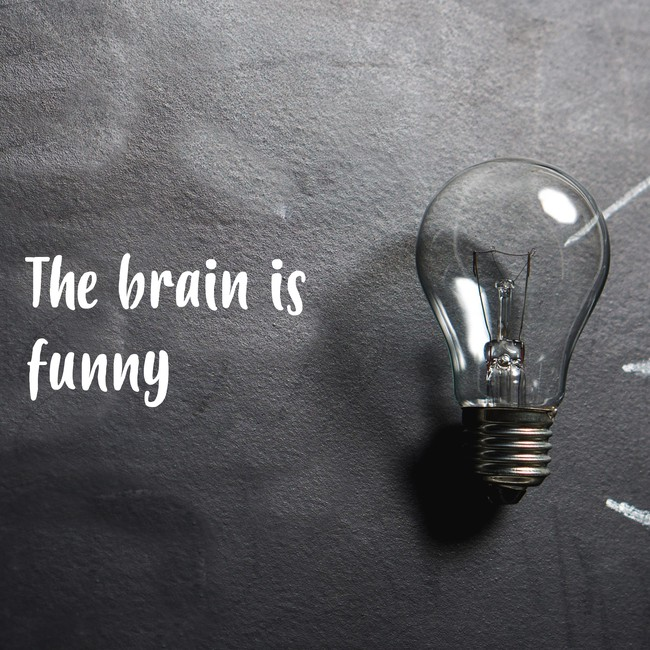
\includegraphics[width=250px]{images/inspirobotQuote.jpg}
  \caption{Quote die von einer \gls{KI} generiert worden ist. \textit{Die Resultate sind noch nicht zufriedenstellend} \cite{inspirobot}}
  \label{fig:Inspirational quote by AI}
\end{figure}
\vspace*{\fill}\clearpage

%% -------------------
%% |   Directories   |
%% -------------------
\tableofcontents
\cleardoublepage

%\listoffigures
%
%\listoftables
%\cleardoublepage

% Glossary


\newglossaryentry{IA}{
	name=IA,
	description=Intelligenter (persönlicher) Assistent
}

\newglossaryentry{KI}{
	name=KI,
	description = Jegliches Programm\, das es einer Maschine erm\"oglicht auf ihre Umwelt zu reagieren.
}

\newglossaryentry{MaschinellesLernen}{
	name = ML,
	description = Maschinelles Lernen\, künstliche generierung von Wissen aus Erfahrung.
}

\newglossaryentry{ANN}{
	name = ANN,
	description = Artificial Neural Network\, ein Künstliches Neuronales Netz.
}

\newglossaryentry{FFN}{
	name = FFN,
	description = Feed Forward Network\, ein Künstliches Neuronales Netz dessen Neuronen einen Azyklischen Graph bilden.
}

\newglossaryentry{FCNN}{
	name = Fully connected Neural Network,
	description = ein Neuronales Netz\, in dem jede Lage mit der nächsten verbunden ist.
}

\newglossaryentry{RNN}{
	name = RNN,
	description = Recurrent Neural Network\, ein Neuronales Netz\, das im gegenzug zu Feed Forward Netzten es erlaubt Signale an vorangehende Schichten zurückzugeben.
}

\newglossaryentry{test}{
name = testosterone,
description = itworks
}

\newglossaryentry{MT}{
name = MT,
description = Machine Translation\, eine automatische Übersetzung von geschriebener oder gesprochener Sprache in eine andere Sprache bzw. Form.
} 

\newglossaryentry{NMT}{
name = NMT,
description = Neural machine translation\, automatische Übersetzung von geschriebener oder gesprochener Sprache in eine andere Sprache bzw. Form mithilfe von Künstlichen Neuronalen Netzen (ANN).
}

\newglossaryentry{NLP}{
name = NLP,
description = natural language programming\, Programmieren in natürlicher Sprache\, z.B Deutsch oder Englisch.
}

\newglossaryentry{Backpropagation}{
	name = Backpropagation,
	description = Ein Werkzeug das es ANN ermöglicht zu trainieren. Weights und Biases werden geupdated.
}

\newglossaryentry{Tensorflow}{
	name = Tensorflow,
	description = Ein Open Source Framework für ANN von Google.
}

\newglossaryentry{Ausreisser}{
	name = Ausreißer,
	description = Ein Funktionswert\, der um ein vielfaches von seinem zeitlich vorgehenden Wert abweicht.
}

\newglossaryentry{Turingtest}{
	name = Turingtest,
	description = ein von Alan Turing entwickelter Test\, ob eine Maschine ein dem Menschen gleichwertiges Denkvermögen hat
	}

%% -----------------
%% |   Main part   |
%% -----------------

%Abstract%
\chapter{Abstract}
[TODO] Ein Abstract ist eine prägnante Inhaltsangabe, ein Abriss ohne Interpretation und Wertung einer wissenschaftlichen Arbeit.
\newpage

\section{\textbf{Einleitung}}
\begin{figure}[h!]
  \center
  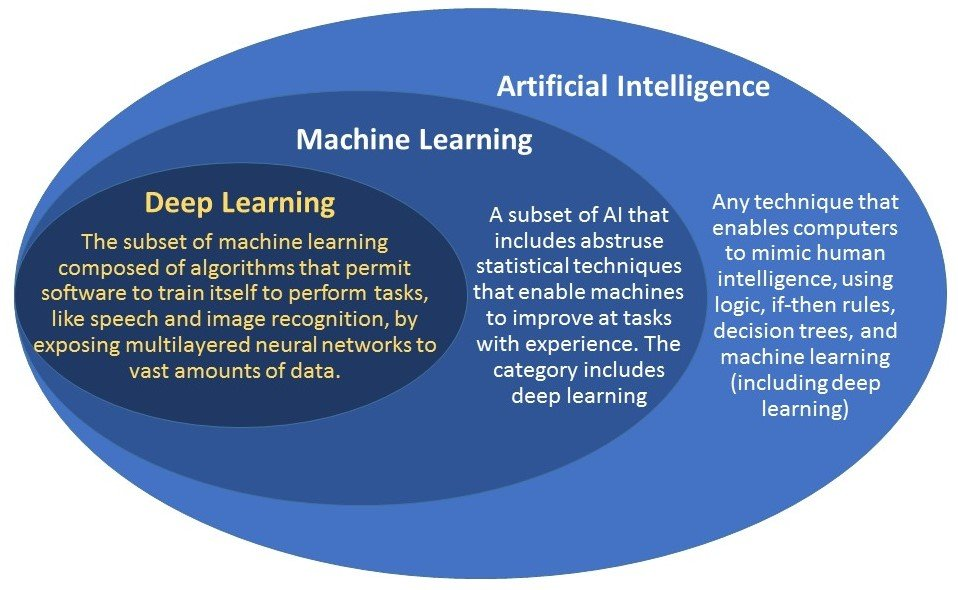
\includegraphics[width=\textwidth]{images/machineLearningInAI.jpg}
  \caption{Veranschaulichung, wie Maschinelles Lernen einzuordnen ist. \cite{machineLearning1}}
  \label{fig:Veranschaulichung, wie Maschinelles Lernen einzuordnen ist.}
\end{figure}

Maschinelles Lernen(\gls{MaschinellesLernen}) ist ein Teilbereich der K\"unstlichen Intelligenz(\gls{KI}). Es handelt sich also um eine Methode, die es Maschinen erm\"oglicht auf ihre Umwelt zu reagieren. Weil es oft schwierig wenn nicht unm\"oglich ist von Hand zu erkennen welche Reaktion das beste Ergebnis liefert versucht man dies Maschinell zu lösen. Dank statistischer Auswertungen k\"onnen Algorithmen entstehen, die mit einer gewissen Wahrscheinlichkeit korrekte Ergebnisse liefern, ohne das der Programmierer sich Gedanken machen muss, wie der Algorithmus letzendlich aufgebaut ist. Diese Methode wird \gls{MaschinellesLernen} genannt.\newline

\subsection{Anwendungen im Bereich der Informatik}
	In jedem Gebiet in dem große Mengen an Daten zur Verf\"ugung stehen bzw. generiert werden können, ist \gls{MaschinellesLernen} theoretisch anwendbar. Weil dies auf so ziemlich jeden Bereich der Informatik zutrifft, erhofft man sich große Fortschritte von dieser neuen Technologie \cite{kour_2018}. \newline
Obwohl die Theorie hinter dieser Art der Datenauswertung seit langem bekannt ist, so finden m\"achtigere Algorithmen die meißt auf Neuronalen Netzen basieren erst seit kurzem verbreitete Anwendung dank verbesserter Rechenleistung. \cite{DBLP:journals/corr/abs-1803-08971} \newline
	\newline Anwendungsbereiche sind zum Beispiel:
\begin{itemize}
	\item Gesichtserkennung
	\item Spamerkennung (Email)
	\item Spracherkennung
	\item Handschrifterkennung
	\item automatische Medikamentenentwicklung
	\item Maschinelle Übersetzungen
\end{itemize}

In dieser Ausarbeitung werden wir uns insbesondere für Künstliche Neuronale Netze (\gls{ANN}) sowie deren Anwendung für Maschinelle Übersetzungen interessieren.

\subsection{Maschinelles Lernen: Ein erstes Beispiel}
	Hören sie sich dieses Beispiel an: \hyperlink{https://www.audioblocks.com/stock-audio/playground-children-playing.html}{audiofile}\newline
	Sie erkennen sofort, das es sich hier um spielende Kinder handelt.
Unser Gehirn schafft es mit extremer Genauigkeit Komplexe Geräusche zu erkennen und zu analysieren. Auch wenn wir nicht erkennen was jedes einzelne Kind ruft, so wissen wir instinktiv das es sich um Kinder handelt.
Schauen wir uns einmal die Wellenfunktion eines Abschnittes dieses Audiofiles an:
\begin{figure}[h!]
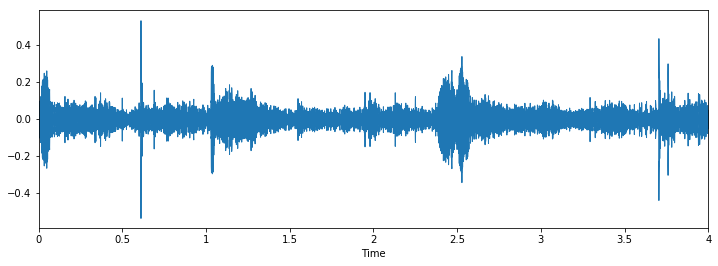
\includegraphics[width=\textwidth]{images/KidsPlaying.png}
  \caption{Audiofile spielender Kinder. Luftdruck/Umgebungsdruck in Funktion der Zeit (Sekunden). \cite{shaikh_faizan_2017}}
  \label{fig:Audiofile Spielende Kinder}
\end{figure}

Vergleichen wir dieses mit der Wellenfunktion eines PressluftHammers:
\begin{figure}[h!]
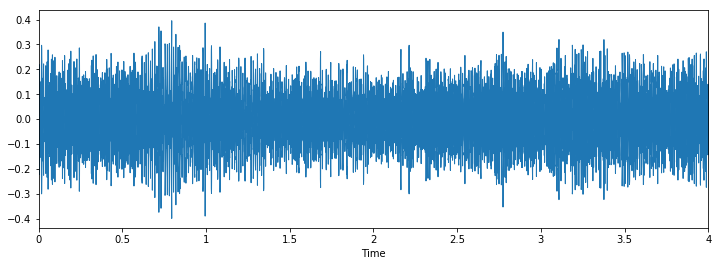
\includegraphics[width=\textwidth]{images/jackhammer.png}
  \caption{Audiofile eines Presslufthammers. Luftdruck/Umgebungsdruck in Funktion der Zeit (Sekunden). \cite{shaikh_faizan_2017}}
  \label{fig:Audiofile pressluftHammer}
\end{figure}

Wir bemerken einige klare Unterschiede. Falls wir nun ein Programm schreiben wollen, das erkennt ob ein Audiofile spielende Kinder oder das Geräusch eines Presslufthammers enthält, so können wir Anhand der Wellenfunktion dieser Geräusche einige Ansätze Folgern. Wir bemerken zum Beispiel, das es bei kreischenden Kindern deutlich mehr Ausreißer gibt als bei dem Geräusch eines Presslufthammers. Wir könnten also ein Programm schreiben, das ein Audiofile nach der Anzahl an Ausreißern pro Zeit(\textbf{APS}) erkennt, d.h. klassifiziert.
\newpage
\begin{lstlisting}
String classify(int[] audiofile) {
   	int APS = getAPS(audiofile); 	// AusreisserProSekunde
	if (APS > (spielkinderDurchschnittsAPS + pressluftHammerDurchschnittsAPS) / 2)){
		return "SpielendeKinder";
	} else {
		return "PressluftHammer";
	}
}
\end{lstlisting}

Man bemerkt jedoch, das man hierfür schon wissen muss, welchen Wert die \textbf{APS} von spielenden Kindern bzw. von Presslufthämmern im Durchschnitt annehmen. Dazu braucht man einen großen Datensatz an Audiodaten, bei denen man weiß um welche Geräusche es sich handelt. Falls diese Vorhanden sind, kann man folgendes Programm schreiben, welches den Durchschnittswert der \textbf{APS} für die jeweilige Kategorie ermittelt:

\begin{lstlisting}
int mittelwertAPS = (spielkinderDurchschnittsAPS + pressluftHammerDurchschnittsAPS) / 2);
    String classify(int[] audiofile, String category) {
        	int APS = getAPS(audiofile);
			if (APS > mittelwertAPS){
				updateAPS(APS, category);		
				return "SpielendeKinder";
			} else {
				updateAPS(APS, category);
				return "PressluftHammer";
			}
    }   
void updateAPS(int APS, String category) {
	if(category.equals(spielendeKinder)) {
		spielendeKinderAPS.add(APS);
	else {
		pressluftHammerAPS.add(APS);
	}
}
\end{lstlisting}

Man bemerkt, das dieses Programm noch immer ermittelt, welcher Kategorie die Audiofiles angehören. Daher kann es, falls bekannt ist um welches der beiden Kategorien es sich handelt weiterverwendet werden. Die Ausreißer pro Sekunde (\textbf{APS}) werden damit mit jedem neuen Audiofile präziser, das Programm Lernt mit der Zeit. Dies ist ein Beispiel sehr rudimentärem \gls{MaschinellesLernen}.\newline
Während dieses Programm sehr einfach ist, so gibt es weitaus mächtigere Programme, in denen der Algorithmus nicht nur den Wert einer Variablen erkennt, sondern auch de Kriterien zur Unterscheidung zwischen Kategorien oder sogar Kategorien selber ermittelt.

\subsection{Aufkommen von Maschinellem Lernen}
Maschinelles Lernen generell und insbesondere Neuronale Netze erfreuen sich seit einigen Jahren \textit{Stand 2018} großer Aufmerksamkeit. Der Grundstein für diese Verfahren wurde jedoch schon Ende des 18. Jahrhunderts von Thomas Bayes gelegt\cite{bayes1763essay}. \newline
Während die ersten Anwendungen zum Großteil abstrakter mathematischer Natur waren\cite{legendre1805nouvelles}, so befasst sich schon 1913 die erste These mit der Analyse von Gedichten\cite{markov2006example}. Dort analysiert Markov ein Gedicht und bemerkt, das man Wahrscheinlichkeiten formulieren kann, welche Eigenschaften weitere Teile vom Text haben ohne das man die Gesamtheit des Gedichtes in Betracht ziehen muss. \newline
1950 formuliert Alan Turing die Turing Learning Machine \cite{machinery1950computing}, ein Jahr später entwickeln und bauen zwei Wissenschaftler das erste neuronale Netz\cite{snarc}. 1957 entwickelt Frank Rosenblatt den "perceptron"\cite{rosenblatt1958perceptron}, ein erstes Modell eines vollständig verbundenem neuronalen Netzes (\gls{FCNN}).

\begin{figure}[H]
  \center
  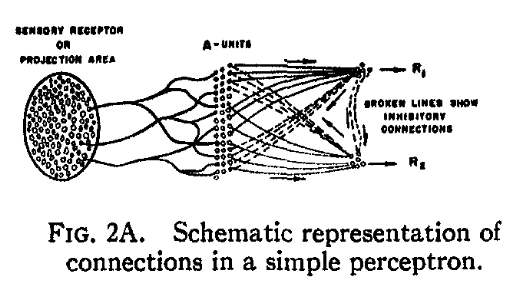
\includegraphics[width=\textwidth]{images/perceptron.png}
  \caption{Zeichnung eines Perceptrons in der ursprünglichen These. \cite{rosenblatt1958perceptron}}
  \label{fig:perceptron}
\end{figure}
1970 wird eine erste Form der Fehlerrückführung (\textit{\gls{Backpropagation}}) entwickelt\cite{linnainmaa1970representation}, 1982 wird ein erstes Rekurrentes Neuronales Netz (\gls{RNN}) entwickelt, welches es ermöglicht Sequenzen von Daten zu verarbeiten, die voneinander abhängen. Anfang des 21. Jahrhunderts und insbesondere ab 2010 hat die Rechnerleistung so sehr zugenommen, das sehr rechenintensive Anwendungen von Maschinellem Lernen möglich werden. Die ersten kommerziellen Bilderkennungssoftware  kommen auf den Markt \cite{taigman2014deepface}. 2016 stellte Google seine Neuronale Maschinelle Übersetzungssoftware vor. Microsoft zieht noch im selben Jahr nach. \cite{microsoftTranslator}
\newline
\newline
Wir werden nun Künstliche Neuronale Netze (\gls{ANN}) kurz einführen.
\section{Künstliche Neuronale Netze (\gls{ANN})}
Ein technischer Durchbruch ist oft \textit{nur} die gelungene Nachahmung eines in der Natur vorkommenden Phänomens. \gls{ANN} werden oft beschrieben als Versuch das menschliche Gehirn nachzubauen. Während diese Unterfangen nicht oder nur teilweise gelungen sind \cite{Adan2018Oct}, haben sich einige Nebenprodukte dieser Forschung als sehr nützlich erwiesen.
Eines dieser Nebenprodukte ist die Entwicklung \gls{ANN}. Es handelt sich dabei um ein Programmiergerüst (\textit{Framework}) für Algorithmen die auf \gls{MaschinellesLernen} basieren. Dieses erlaubt Eingabesignale, die verarbeitet werden zu mehreren Ausgabesignalen. Beschrieben werden \gls{ANN} mit Begriffen aus der Biologie. Die erste Lage(\textit{inputlayer}), besteht aus einer gewissen Anzahl an Knoten, sogenannten \textit{Neuronen}, die bei unterschiedlichen Eingaben unterschiedlich aktiviert werden. Diese sind mit weiteren Neuronen über sogenannte \textit{Synapsen} verbunden und versenden je nach \gls{ANN} mehr oder weniger starke Signale über diese Verbindungen.
%image of a Fully connected Neural Network%
\begin{figure}[H]
  		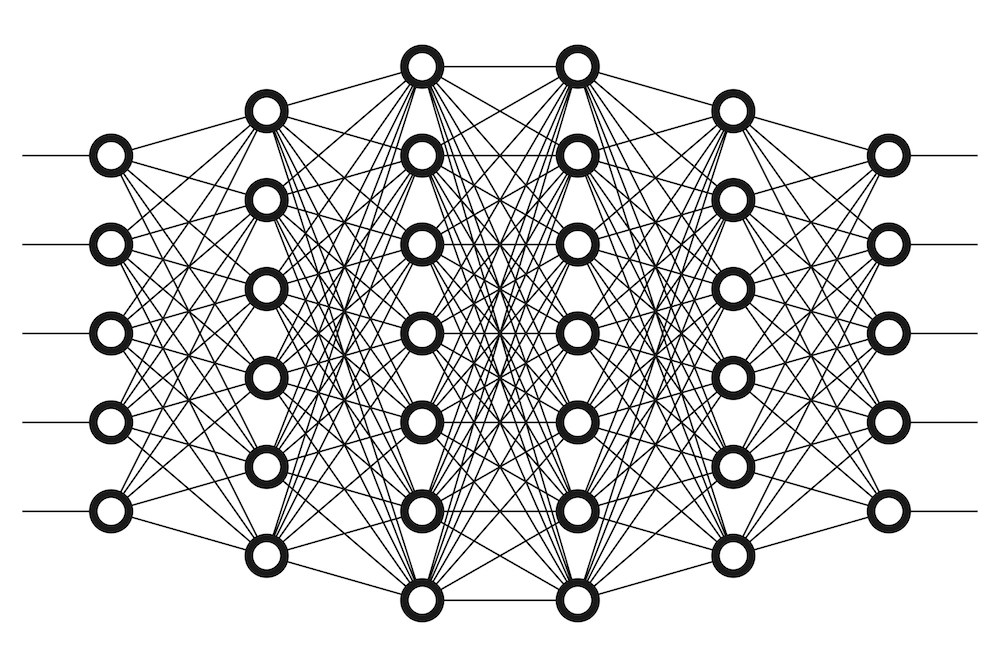
\includegraphics[width=\linewidth]{images/DeepNeuralNetwork.jpg}
  		\caption{Topologie eines \gls{FCNN}. 	\cite{NeuronalesNetzImage} }
  		\label{fig:Neuronales Netz}
\end{figure}

Neuronen können in Lagen(\textit{Layers}) zusammengefasst werden, welche die Stufen des \gls{ANN} darstellen, die mithilfe der Breitensuche bestimmt werden können.

Wie in unserem Beispiel erwähnt, ist das Ziel von neuronalen Netzen Eigenschaften zu erkennen, die gewisse Objekte gemeinsam haben. \gls{ANN} sollen:
\begin{itemize}
	\item Klassifizieren
	\item Zusammenhänge erkennen
\end{itemize}
\subsection{Aktivierungsfunktion}
Durch Signale können Neuronen im \gls{ANN} mehr oder weniger stark aktiviert werden. Das Ausgabesignal eines aktivierten Neurones wird durch die Aktivierungsfunktion berechnet. Diese bildet den Aktivierungswert auf ein Intervall ab und ist daher eine nichtlineare Funktion. Ohne diese Funktion könnten komplexe nichtlineare Datensätze wie Bilder, Videos sowie Audio nicht analysiert werden.
\newline 
\newline
\textit{''Neural-Networks are considered Universal Function Approximators. It means that they can compute and learn any function at all. Almost any process we can think of can be represented as a functional computation in Neural Networks.'' \cite{walia_2017}} 
\newline [KANN ICH DAS SO STEHEN LASSEN ODER MUSS ICH ES ÜBERSETZEN? FINDE DAS DAS ZITAT EIGENTLICH SEHR SCHÖN BESCHREIBT WELCHE FUNKTION DIE AKTIVIERUNGSFUNKTION BESITZT]
\newline
Eine früher beliebte Aktivierungsfunktion war die normalisierte Sigmoid Funktion. 
\begin{align*}
f(x) &= \frac{1}{1 + e^{-x}}
\end{align*}
Während dies die wohl allgemein bekannteste Aktivierunngsfunktion ist, verwenden moderne \gls{ANN} heute eine Variante der \textit{Rectifier Funktion}\cite{lecun_bengio_hinton_2015}:
\begin{align*}
f(x) &= max(0, x)
\end{align*}
Die eine beliebte Approximierung dieser Funktion ist z.B die analytische Funktion:
\begin{align*}
g(x) &= log(1 + e^{x})
\end{align*}
Die \textit{Rectifier Funktionen} besitzt einige entscheidende Vorteile, weshalb sie heute so weit verbreitet ist. sie sind leicht ableitbar, sind einfach zu berechnen (\textit{d.h. sie benötigen wenig Rechenleistung}) und besitzen einige weitere Eigenschaften die sehr hilfreich sind beim trainieren von \gls{ANN}.


\subsection{Propagation function}

Jede Verbindung besitzt eine Gewichtung, \textit{weight}. Diese beschreibt wie viel Einfluss sie hat auf die Aktivierung des verbundenen Neurons.

Die \textit{propagation function} berechnet den Input $p_j(t)$ des Neurones j anhand der Outputs $o_i(t)$ der vorangehenden Neuronen.
\begin{align*}
p_j(t) &= \sum_{i}^{} o_i(t) w_{ij}
\end{align*}
Um eine Aktivierungsschwelle (\textit{threshold}) einzuführen kann ein sogenannter \textit{bias} der Summe hinzugefügt werden. Dies ist nötig wenn ein Neuron nur ab einem bestimmten Aktivierungswert von Bedeutung ist.
\begin{align*}
p_j(t) &= \sum_{i}^{} o_i(t) w_{ij} + bias
\end{align*}
Ein großer Vorteil von \gls{ANN} ist, das sie als eine Folge von Matrixmultiplikationen darstellbar sind, welche besonders effizient durch Computerprozessoren berechnet werden können.
\begin{center}
\begin{figure}[H]
  		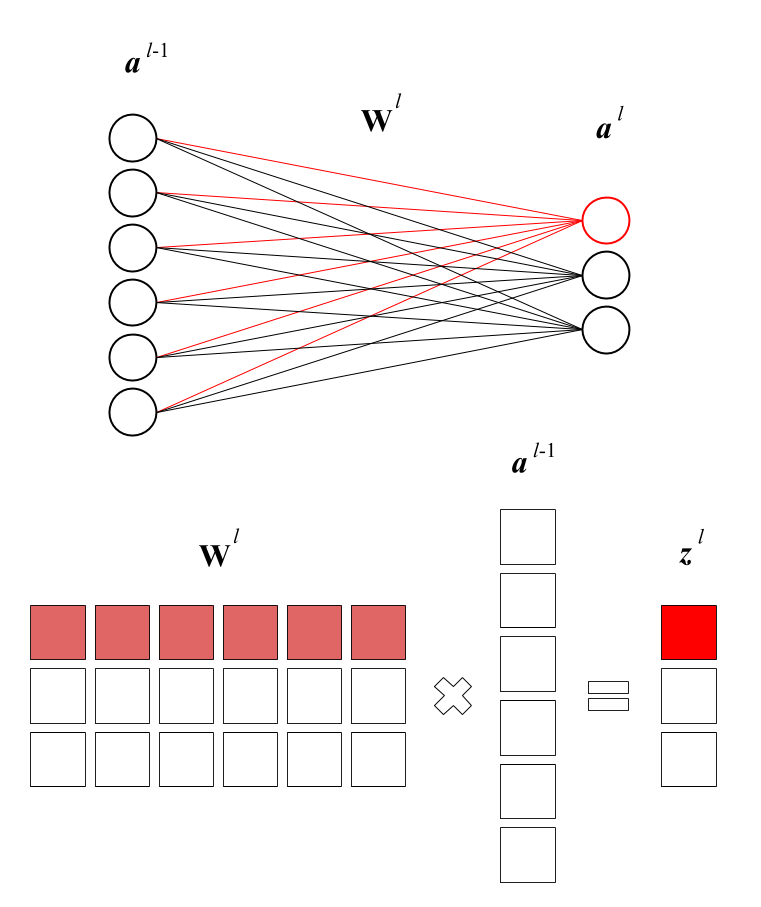
\includegraphics[scale=0.4]{images/NNMatrix.png}
  		\caption{Neuronales Netz in Matrixrepresentation. Hierbei ist $a^{l} = f(z^{l})$ wobei $f$ die Aktivierungsfunktion darstellt. \cite{hallstroem_2016}}
  		\label{fig:Matrixrepresentation eines Neuronalen Netzes}
\end{figure}
\end{center}

%\subsection{Fully Connected Layers}
%\subsection{Convolution}
%\subsection{Pooling}
%\subsection{Reccurence}
\subsection{Training eines \gls{ANN}}
Wie zuvor beschrieben, benötigt ein \gls{ANN} massive Datensätze. Gesucht wird nun ein Algorithmus der anhand dieser Daten die \textit{weights} und \textit{biases} so einstellt, das das Netzwerk seine Funktion erfüllt. 
Einer dieser Algorithmen ist die Fehlerrückrührung (\textit{Backpropagation}).

\subsubsection{Backpropagation}
Der Backpropagation Algorithmus verläuft folgendermaßen: Erst wird ein Eingabemuster durch das \gls{ANN} propagiert. Daraufhin wird die Ausgabe des Netzes, d.h. die Aktivierung des letzten Layers verglichen mit der gewünschten Aktivierung. Der Fehler des Netzes kann durch die quadrierte Fehlerfunktion berechnet werden.
\begin{align*}
E_j &= \dfrac{(t_j - y_j)^2}{2}
\end{align*}
\textit{$t_j$ ist der gewünschte Output des Neurons j} \newline
\textit{$y_j$ ist der wirkliche Output des Neurons j}		\newline


Das Ziel ist es nun die Summe der Fehlerfunktionen über alle möglichen Inputs zu minimieren. Dies ist nicht möglich ohne alle möglichen Kombinationen von \textit{weights} und \textit{biases} auszuprobieren, jedoch kann man dank des Gradientenverfahrens lokalen Minimas nahe kommen.

\subsubsection{Gradientenverfahren}



\subsection{Limitationen und Gefahren von Neuronalen Netzen}
Währen \gls{ANN} im Moment großer Beliebtheit genießen, so sollte man sich einiger ihrer Nachteile bewusst sein. Wie zuvor erwähnt wird durch das Gradientenverfahren nur lokale Minima gefunden, das die Performance eines \gls{ANN} nach dem Trainieren ist daher stark vom Anfangszustand abhängig und kann unter Umständen auf enttäuschendem Niveau trotz neuer Daten stagnieren. Das trainieren von \gls{ANN} ist noch immer sehr Rechnerleistungsintensiv und benötigt große Mengen an Daten (\text{labeled data}). \newline Durch diese neuen Technologien sind Daten sehr wertvoll geworden. Sie sind der Grund weshalb Suchmaschinen und Soziale Netzwerke zu den Wertvollsten unternehmen Weltweit gehören. Während \gls{MaschinellesLernen} zwar nicht verantwortlich ist für den unvorsichtigen Umgang und Handel mit unseren Daten, so verstärken sie diesen Trend. entstehende Kontrollverlust der durch das nutzen solcher Werkzeuge entsteht. Es wird oft angenommen, das es nicht möglich ist ein \gls{ANN} zu verstehen, das es sich um eine \textit{black box} handelt. Diese Aussage sollte relativiert werden, es ist in den Letzten Jahren viel geforscht worden um dieses Problem zu überwinden\cite{lime}. Nichtsdestotrotz ist es noch immer schwierig das Innere eines \gls{ANN} oder ähnlichem Konstrukt zu verstehen, es muss immer damit gerechnet werden, das ein Neuronales Netz auf völlig unvorhergesehen Weise auf eine Neue Eingabe reagiert. Es können kaum Garantien für das Verhalten eines neuronalen Netzes gegeben werden. Es ist daher mehr als problematisch diese Algorithmen für Zwecke zu nutzen in denen über Menschenleben entschieden wird, wie es das Pentagon mit Google's Framework \gls{Tensorflow} getan hat \cite{gibbs_2018}. Anwendungen von \gls{ANN} werfen ethische Fragen auf und es sollte immer Abgewogen werden, in welchen Fällen man auf \gls{ANN} lieber verzichten sollte.

Trotz dieser Bedenken hat Maschinelles Lernen schon große Fortschritte in vielen Bereichen der Informatik ermöglicht. Im Bereich der Programmierung in Natürlicher Sprache sind diese schon längst beim Nutzer angekommen in der Form von Chatbots oder persönlichen Assistenten wie Siri im Jahre 2010.

\section{Maschinelle Übersetzungen (\gls{MT})}

 Während Chatbots noch weit entfernt sind den Turingtest zu bestehen, so haben Maschinelle Übersetzungen dank \gls{ANN} von und ins Englische quasi Menschliche Fehlerraten erreicht\cite{googleaiblog_2016}.
 
\begin{figure}[H]
  \center
  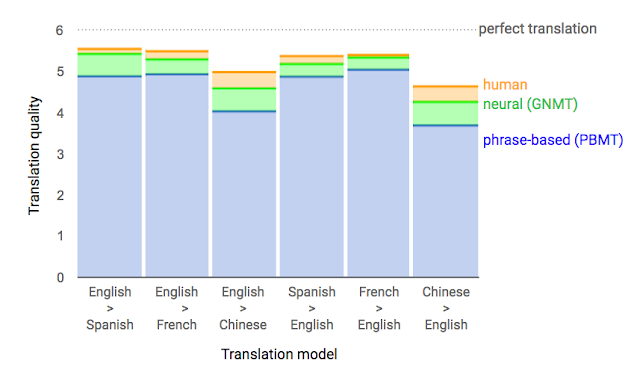
\includegraphics[width=\textwidth]{images/MTGoogle.png}
  \caption{Google Translate Performance. Muttersprachler wurden gebeten Übersetzungen von Google Translate auf einer Skala von 0 bis 6 zu bewerten. \cite{googleaiblog_2016}}
  \label{fig:GoogleTranslate Performance}
\end{figure}

\subsection{Neuronale Maschinenübersetzung (\gls{NMT})}
\gls{NMT} hat signifikative Verbesserungen in \gls{MT} ermöglicht. Dank \gls{ANN} behauptet Google z.B. ihre Fehlerraten um 60\% gesenkt zu haben \cite{wu2016google}. Andere Dienste wie Microsoft sowie Yahoo melden ähnliche Fortschritte \cite{Microsoft2018}.
%\begin{itemize}
	%\item Recurrent Neural Networks
		%[Warum gerade diese?]
		%[Elman Network, Jordan Netzwerk, Hopfield Network,...]
	%\item 
%\end{itemize}

\subsection{Kuriositäten}

Algorithmen die auf \gls{MaschinellesLernen} und insbesondere auf \gls{ANN} basieren ist oft unvorhersehbar und können kuriose Lösungswege nutzen.
\begin{itemize}
	\item Facebook Chatbots haben eine eigene Sprache erfunden um zu kommunizieren\cite{wilson_2018}.
	\item Google Translate hat eine Sprache erfunden die als Zwischensprache dient \cite{googleAiblog_2016Translation}.
\end{itemize}
Facebook hat zwei Chatbots verschiedene virtuelle Objekte gegeben, welche einen bestimmten Wert besitzen, die diese miteinander austauschen konnten. Die Verhandlungstaktiken die die beiden Chatbots nutzen sollten durch \gls{MaschinellesLernen} erlernt werden.

\begin{figure}[H]
  \center
  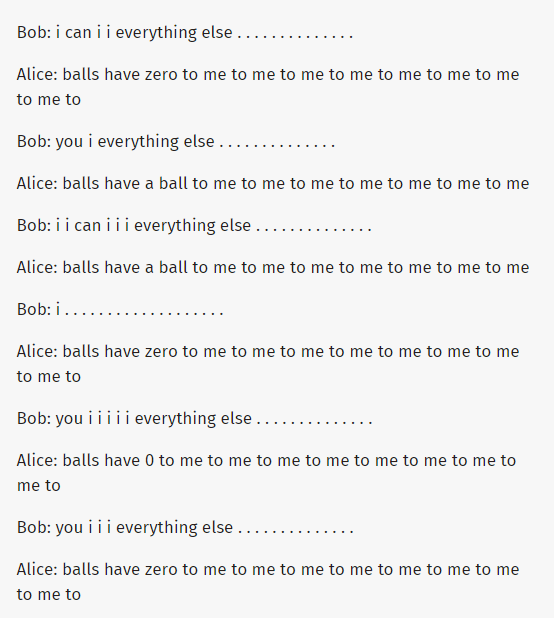
\includegraphics[scale=0.6]{images/FacebookChatbots.png}
  \caption{Facebook Chatbots entwickeln ihre eigene Sprache. \cite{wilson_2018}}
  \label{fig:Facebook Chatbots}
\end{figure}

Das die Chatbots beschließen nicht mehr auf Englisch zu Kommunizieren hatte niemand vorausgesehen. Es zeigt auf wie unvorhergesehen sich \gls{MaschinellesLernen} Algorithmen verhalten können.
\newline
\newline
Bevor Google translate \gls{ANN} verwendete, wurde jeder Satz erst ins Englische und dann in die Zielsprache übersetzt. Diese Methode limitiert die Anzahl an Übersetzungen die Programmiert werden müssen drastisch, schlägt jedoch fehl sobald das Wort das übersetzt werden muss nicht im englischen vorkommt. Das \gls{ANN} das von Google seit kurzem eingesetzt wird hat eine eigene Sprache entwickelt. Jeder Satz wird nun erst in die entwickelte Sprache übersetzt und dann in die Zielsprache. In dieser Sprache gibt es ein Wort für Baum. Dieses ist verlinkt mit jedem Wort in jeder Sprache, das Baum bedeutet. Man bemerkt das das neuronale Netz denselben Ansatz verwendet hat, den Menschen zuvor auch angewandt haben, jedoch ein Schritt weiter gegangen ist.

\section{\textbf{Bewertung}}
\gls{MaschinellesLernen} ist ein mächtiges Werkzeug in vielen Bereichen der Informatik. Insbesondere \gls{ANN} und ähnliche Algorithmen haben die allgemeine Meinung das Menschen in gewissen Bereichen immer besser als Maschinen sein werden zumindest in Teilen widerlegt. Dadurch das diese Algorithmen Erfahrung sammeln und somit Lernen, stehen sie Menschen in Problemlösungen theoretisch in nichts nach.\newline
Jedoch besitzen diese Werkzeuge dieselben Probleme die wir Menschen auch haben. Sie sind nur so gut wie die Daten die ihnen als Training zur Verfügung gestellt werden, genaue Lösungswege sind nur schwer zu durchschauen. In gewissen Bereichen, wie der \gls{MT} sind diese Probleme nicht von Relevanz, Sprachen verändern sich ständig mit der Zeit, daher ist es wichtig, das Übersetzungstools genauso \textit{mit ihrer Zeit gehen} d.h. sich dem Allgemeinen Sprachgebrauch anpassen. Maschinelles Lernen bietet Lösungen für sich dynamisch verändernde Probleme an. Man muss sich jedoch immer der Schwächen und Gefahren dieser Algorithmen bewusst sein sowie abwägen in welchen Fällen man auf sie verzichten sollte.
\mainmatter
\pagenumbering{arabic}

%% --------------------
%% |   Bibliography   |
%% --------------------
\cleardoublepage
\phantomsection
\addcontentsline{toc}{chapter}{\bibname}

\iflanguage{english}
{\bibliographystyle{IEEEtranSA}}	% english style with numeric references
{\bibliographystyle{alphadin}}	% german style

\bibliography{thesis}


%% ----------------
%% |   Appendix   |
%% ----------------
%\cleardoublepage
%%% appendix.tex
%%

%% ==============================
%\chapter{Appendix}
%\label{ch:Appendix}
%% ==============================

\appendix

\iflanguage{english}
{\addchap{Appendix}}	% english style
{\addchap{Anhang}}	% german style


...



%% ----------------
%% |   Glossary   |
%% ----------------
\cleardoublepage
\printglossary

\end{document}
